\documentclass[]{article}
\author{Diego Biagini}
\title{Valutazione prestazioni algoritmi di sorting}

\usepackage[utf8]{inputenc}
\usepackage[margin=3cm]{geometry}
\usepackage{algorithmic}
\usepackage{algorithm}
\usepackage{graphicx}
\floatname{algorithm}{}

\graphicspath{{../plots/}}

\begin{document}
\maketitle
\newpage
\section{Introduzione}
Una delle classi di problemi più studiate nel campo dell'informatica sono i problemi di ordinamento.
Essi possono essere descritti nel seguente modo:\\ a partire da una sequenza di dati 
$S = \{x_1, ... , x_n\}$ in ingresso trovare una permutazione $S^{\prime} = \{x_1^{\prime}, ... , x_n^{\prime}\}$ di essa tale che $x_1^{\prime} \leq x_2^{\prime} \leq ... \leq x_n{\prime}$.\\
Per la loro risoluzione sono stati pensati numerosi algoritmi di ordinamento,questi differiscono soprattutto per i campi di applicazione e per il comportamento rispetto a certe sequenze di ingresso.\\
Per valutare quale sia meglio usare è quindi necessario vedere quanto sono efficienti, ovvero quanto tempo impiegano ad essere eseguiti, rispetto a insiemi di dati particolari e con dimensione sempre crescente.\\
Gli algoritmi che saranno presi in esame sono \textbf{Insertion sort} e \textbf{Quicksort}.


\section{Cenni teorici}

\subsection{Tempo di esecuzione di un algoritmo}
Nell'analizzare un qualsiasi algoritmo emerge la necessità di definire in modo chiaro le sue prestazioni, senza essere vincolati a fattori come la macchina su cui viene eseguito.\\ Per questo motivo supponiamo sempre che essi siano eseguiti su una \textbf{RAM(Random access machine)}, una macchina astratta con le seguenti caratteristiche:
\begin{itemize}
\item può essere eseguita solo un'operazione alla volta(macchina monoprocessore)
\item operazioni elementari eseguite in tempo costante
\item infinite celle di memoria di dimensione finita
\end{itemize}
I parametri che di norma vengono presi in considerazione per valutare l'efficienza sono il tempo di esecuzione(misurato in numero di operazioni elementari effettuate) e la quantità di memoria impiegata.\\
\\
Nel caso di algoritmi il cui scopo è analizzare e modificare grandi quantità di dati, come quelli di ordinamento, c'è bisogno di vedere come questi parametri si comportano all'aumentare della quantità di dati presi in esame.\\
Per far questo viene usata la \textbf{notazione asintotica}, attraverso essa siamo in grado di descrivere un limite stretto($\Theta$),superiore($O$) o inferiore($\Omega$) di una funzione al tendere di uno dei suoi parametri all'infinito.\\
Per esempio $f(n) = \Theta(n^2)$ indica che $f$ si comporta come una parabola quando n( il numero di elementi da ordinare nel nostro caso) tende ad infinito, non ci preoccupiamo dei termini di primo o secondo grado.

\newpage
\subsection{Insertion sort}
Insertion sort è un algoritmo di ordinamento iterativo utile soprattutto per ordinare insiemi con un numero ridotto di elementi.

Lo pseudocodice è il seguente:\\
\begin{algorithm}
\caption{Insertion-Sort(A)}
\begin{algorithmic}[1]
\FOR{$j\leftarrow2$ to $A.lenght$} 
	\STATE $key \leftarrow A[j]$
	\STATE $i \leftarrow j - 1$
	\WHILE{ $ i > 0 $ \AND  $A[i] > key$}
		\STATE	$A[i+1] \leftarrow A[i]$
		\STATE $ i \leftarrow i - 1$
	\ENDWHILE
	\STATE $ A[i+1] \leftarrow key$
\ENDFOR 
\end{algorithmic}
\end{algorithm}
\\
La correttezza dell'algoritmo può essere dimostrata con la sua invariante di ciclo:\\ prima della j-esima iterazione il sotto-array $A[1 ... j-1]$ è ordinato e contiene tutti i valori che vi erano presenti inizialmente.\\
E' facile verificare che il caso migliore di questo algoritmo si ha quando l'array dato è già ordinato, infatti in questo caso non entreremo mai nel ciclo while interno.\\
Da questo possiamo dire che nel \textbf{caso migliore} insertion sort è un $\Theta(n)$.\\
Il \textbf{caso peggiore} si ha invece quando l'array è ordinato in senso decrescente, in questo caso il ciclo while controllerà tutti i valori precedenti a j e il tempo di esecuzione asintotico è $\Theta(n^2)$.\\
Il caso medio ha un comportamento simile al caso peggiore,infatti mediamente metà elementi di $A[1 ... j-1]$ sono più piccoli di $A[j]$, nonostante questo abbiamo sempre un comportamento quadratico e possiamo dire che anche nel \textbf{caso medio} insertion sort è un $\Theta(n^2)$
\subsection{Quicksort}
Quicksort è un algoritmo di ordinamento ricorsivo che segue la filosofia divide-et-impera.\\
\'E uno degli algoritmi più usati in virtù delle buone prestazioni che offre quando è eseguito su insiemi di elementi senza un particolare ordine preesistente.\\
Lo pseudocodice dell'algoritmo è il seguente:

\begin{algorithm}
\caption{partition(A,p,r)}
\begin{algorithmic}[1]
\STATE $x \leftarrow A[p]$
\STATE $i \leftarrow p-1$
\FOR{$j \leftarrow p$ to $r-1$}
	\IF{$A[j] \leq x$}
		\STATE $i \leftarrow i + 1$
		\STATE $A[i] \leftrightarrow A[j]$
	\ENDIF
\ENDFOR
\STATE $A[i+1] \leftrightarrow A[r]$
\STATE return $i+1$
\end{algorithmic}
\end{algorithm}
\newpage
\begin{algorithm}
\caption{Quick-Sort(A,p,r)}
\begin{algorithmic}[1]
\IF{$p < r$}
	\STATE $q \leftarrow partition(A,p,r)$
	\STATE $Quick\mbox{-}Sort(A,p,q-1)$
	\STATE $Quick\mbox{-}Sort(A,q+1,r)$
\ENDIF
\end{algorithmic}
\end{algorithm}

Il \textbf{caso migliore} di quicksort si ha quando ad ogni chiamata di partition q si trova esattamente nel mezzo dell'array. In questo caso quicksort ha un comportamento simile a merge sort ed ha un tempo di esecuzione asintotico di $\Theta(nlog(n))$.\\
Il \textbf{caso peggiore} si ha invece quando l'array è già ordinato(caso molto comune) e la divisione dell'array tramite il partition è la peggiore possibile. Il tempo è $\Theta(n^2)$.\\
\'E possibile rimediare questo problema imponendo un ordinamento casuale dell'array in ingresso.\\
Il motivo per cui quicksort è usato frequentemente è il suo comportamento nel \textbf{caso medio}, infatti è possibile dimostrare che esso si avvicina più al suo caso migliore piuttosto che al peggiore e quindi ha un tempo di esecuzione di $\Theta(nlog(n))$.\\
\section{Esperimenti svolti}
Vogliamo testare come gli algoritmi insertion sort e quicksort si comportano all'aumentare della dimensione dei dati da ordinare e sotto certi input, ovvero quanto tempo impiegano per essere eseguiti.\\
Per questo, entrambi gli algoritmi saranno eseguiti su insiemi:
\begin{itemize}
\item casuali
\item corrispondenti al caso migliore
\item corrispondenti al caso peggiore
\end{itemize}

La dimensione degli insiemi da ordinare sarà incrementata esponenzialmente.\\
Iniziamo quindi ordinando un certo tipo di insieme di dimensione pari a 1 con un algoritmo, continuiamo quindi a generare nuovi insiemi di quel tipo di dimensione doppia finchè l'algoritmo non impiega più di qualche minuto(indicativamente 3 minuti) per terminare l'ordinamento.\\
\'E stato scelto di raddoppiare la dimensione degli insiemi dopo ogni test, piuttosto che moltiplicarla per 10, in modo che il tempo di esecuzione tra un test e il successivo non sia troppo diverso.\\
Questo comportamento si noterebbe soprattutto nel caso peggiore di insertion sort, una decuplicazione della dimensione comporta infatti un tempo di esecuzione(teorico) cento volte superiore al precedente.\\
Infine la procedura di testing sarà eseguita sullo stesso insieme di dati(con permutazione casuale) per entrambi gli algoritmi, in modo da vedere effettivamente quale è più performante su uno stesso problema.\\\\
Dato che questi esperimenti saranno eseguiti su una macchina reale sarà necessario imporre alcune limitazioni.\\
Per prima cosa un algoritmo ricorsivo come quicksort in realtà non può richiamarsi all'infinito nella realtà, deve sottostare alla dimensione massima dello stack delle chiamate. Quindi gli esperimenti su questo algoritmo saranno interrotti nel caso in cui non sia possibile richiamare ulteriormente la funzione.\\
Con il caso migliore dell'insertion sort sorge invece un altro problema, data la sua velocità di esecuzione veramente alta ben presto la memoria del calcolatore verrà pienata a forza di aumentare le dimensioni dell'array. Quindi per questo esperimento sarà stabilitò un tempo di esecuzione massimo inferiore rispetto agli altri.\\
\section{Documentazione del codice}
\begin{verbatim}
insertion_sort(array)

quick_sort(array)
quick_sort_rec(array, start, end)
partition(array, start, end)
\end{verbatim}
Gli algoritmi di ordinamento e le loro funzioni accessorie. Entrambi ricevono un array da ordinare e non restituiscono valori.
\begin{verbatim}
get_random_array(size,min_value,max_value)
get_random_asc(size)
get_random_desc(size)
get_random_nodup(size)
get_quick_best_case(size)
\end{verbatim}
Funzioni che data una dimensione generano e restituiscono un array di quella dimensione con certe caratteristiche. In ordine esse servono a creare un array:
\begin{itemize}
\item casuale con elementi compresi tra un minimo e un massimo
\item ordinato in ordine crescente
\item ordinato in ordine decrescente
\item casuale senza elementi duplicati
\item in modo che coincida col caso migliore di quicksort
\end{itemize}
\begin{verbatim}
next_size(current_size)
\end{verbatim}
Data la dimensione attuale di un array restituisce la prossima dimensione da testare.
\begin{verbatim}
test_sorting(max_time, sorting_f, random_array_f, save_to_file, filename)
\end{verbatim}
Si occupa di testare un algoritmo di sorting.\\
Prende come parametri il tempo massimo di esecuzione, la funzione che implementa l'algoritmo da testare, la funzione che genera l'array del tipo voluto. Consente inoltre di salvare i risultati su file se save\_to\_file è impostato a True.\\
Restituisce una lista di tuple, ogni tupla  composta dalla dimensione testata e dal tempo di esecuzione per la data dimensione.
\begin{verbatim}
test_both(max_time,save_to_file)
\end{verbatim}
Testa sia insertion sort che quicksort finchè uno dei due non impiega più di max\_time per essere completato.
\begin{verbatim}
plot_and_save(title, results)
plot_and_save_both(title, results)
\end{verbatim}
Tracciano il grafo dimensione-tempo voluto e lo salvano su file.
\section{Risultati sperimentali}
\subsection{Insertion sort}
\begin{center}
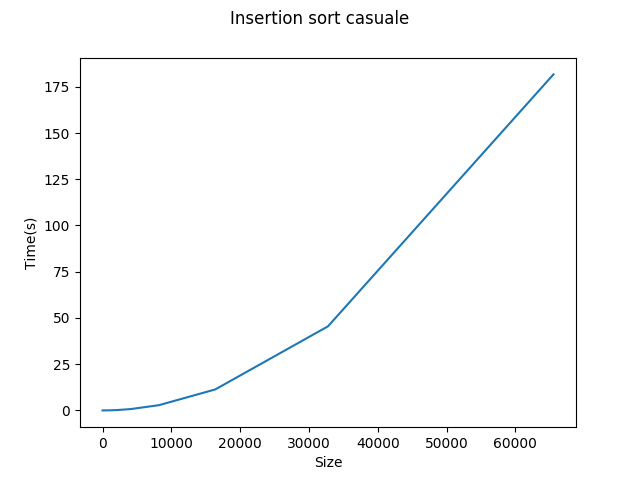
\includegraphics[scale=0.5]{InsertionSortCasuale}\\
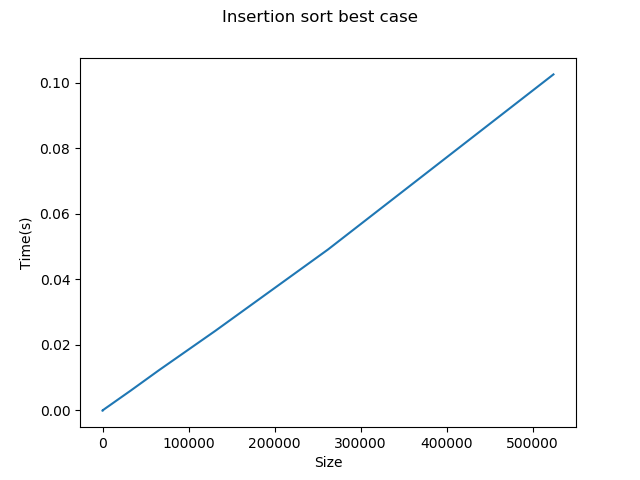
\includegraphics[scale=0.5]{InsertionSortBestCase}\\
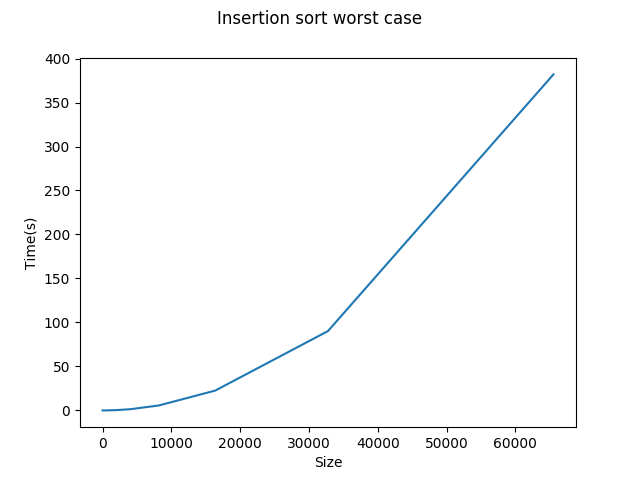
\includegraphics[scale=0.5]{InsertionSortWorstCase}\\
\end{center}

\subsection{Quicksort}
\begin{center}
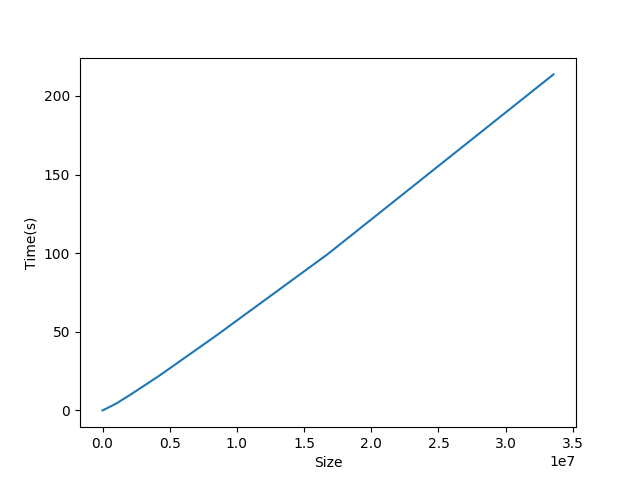
\includegraphics[scale=0.5]{QuickSortCasuale}\\
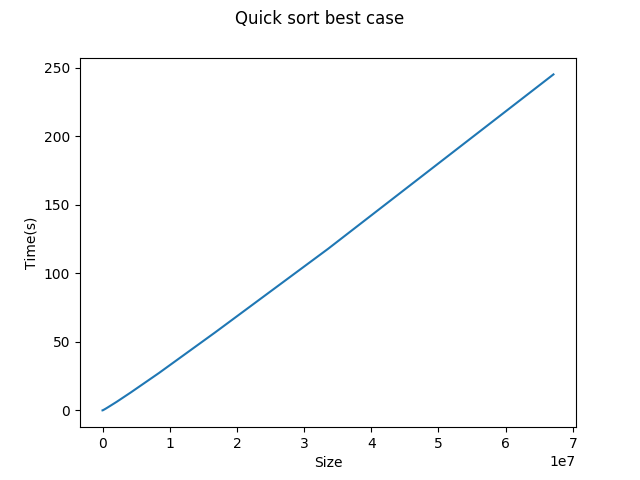
\includegraphics[scale=0.5]{QuickSortBestCase}\\
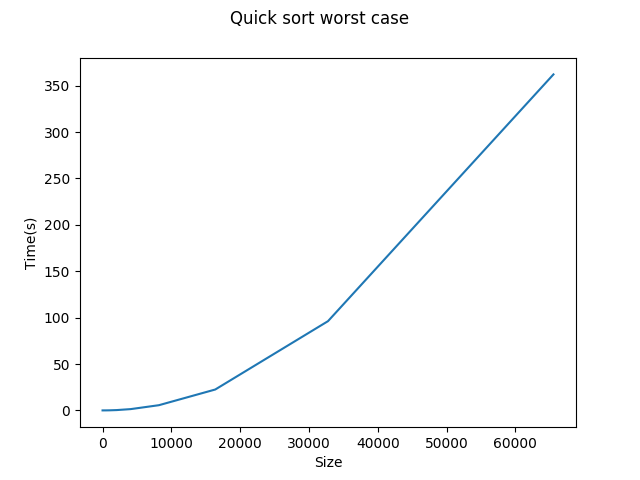
\includegraphics[scale=0.5]{QuickSortWorstCase}\\
\end{center}

\subsection{Entrambi gli algoritmi}
\begin{center}
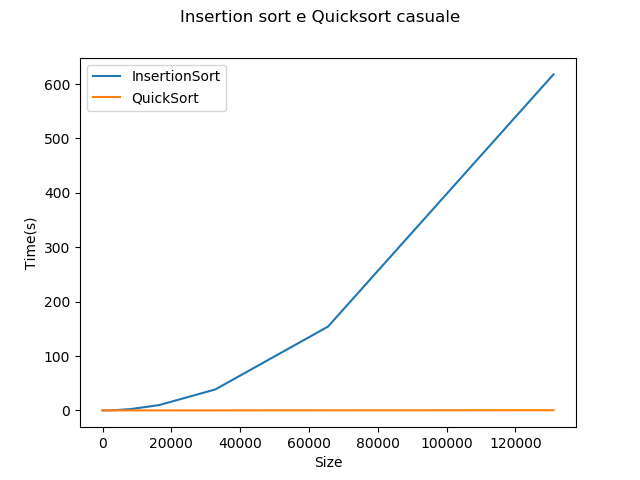
\includegraphics[scale=0.5]{InsertionSortEQuicksortCasuale}\\
\end{center}

\section{Analisi e conclusioni}
Analizzando i risultati degli esperimenti è possibile verificare ciò che ci dice la teoria.\\\\
Riguardo insertion sort, grazie ai grafici tracciati, possiamo vedere come il caso medio e peggiore si avvicinano a delle parabole, mentre il caso migliore è una retta quasi perfetta che riesce ad "ordinare" insiemi di dati veramente velocemente.\\
Nonostante questo,il caso migliore è un caso così particolare(array già ordinato) che non capita molto frequentemente nei problemi di ordinamento classici, non possiamo quindi considerarlo veramente un punto forte dell'algoritmo in applicazioni generiche.\\\\
Dai grafici di quicksort possiamo invece vedere come il caso peggiore sia una parabola, comparabile col caso medio e peggiore di insertion sort, mentre il caso medio e migliore si avvicinano a una retta, nonostante la teoria ci dica che il costo asintotico è $\Theta(nlog(n))$.\\
Quest'ultima cosa ci mostra graficamente come le costanti di quicksort omesse nella notazione asintotica sono veramente piccole, quasi da far apparire il tempo di esecuzione come lineare.\\
Apparentemente l'unico problema di quicksort è il caso peggiore,che è un caso che si può verificare facilmente. \'E possibile rimediare a questo problema implementando $randomized\mbox{-}quicksort(A)$ , questa prima di chiamare l'algoritmo impone una permutazione casuale ad A. In questo modo si può dire che il costo di randomized-quicksort è pari al costo medio di quicksort per ogni sequenza in ingresso.\\\\
Infine esaminando il confronto diretto tra i due algoritmi è evidente la maggiore efficienza di quicksort, che arriva ad essere centinaia di volte più veloce di insertion sort.\\
Un punto a favore di insertion sort può essere la maggior facilità di esecuzione su insiemi di dati veramente grandi, situazione in cui la natura ricorsiva di quicksort è uno svantaggio.\\\\
In conclusione quicksort è l'algoritmo preferibile nella quasi totalità delle applicazioni, nonostante questo insertion sort ha comunque delle applicazioni reali.\\
Un esempio può essere un insieme di dati dinamico, in cui vengono aggiunti spesso degli elementi che non modificano troppo la struttura dell'insieme. In un caso come questo abbiamo un insieme quasi sempre ordinato a meno di qualche elemento, caso in cui insertion sort ha un comportamento quasi lineare.
\end{document}